\documentclass[main.tex]{subfiles}
\begin{document}

\chapter{Implementation}
To ensure a uniform comparison of the algorithms selected in the concept, the external circumstances
must be identical for each algorithm. This chapter will detail the implementation thereof.

\section{System Setup}
It is necessary to perform all experiments on the same machine to ensure a consistent comparison.
We implement all algorithms and further architecture on a Lenovo IdeaPad 5 Pro,
which runs Linux Ubuntu 20.04.5. The laptop has an AMD Ryzen 7 5800H CPU and 16 GB of RAM.

We install the most recent ROS distribution, \textit{ROS Noetic Ninjemys}, as well as \textit{realsense-ros} with all additional dependencies.

% FIXME I think those footnotes with links were a bad idea

\section{Plane Detection Algorithms}
We implement RSPD and OPS using their respective open source implementations on GitHub\footnote{\href{https://github.com/abnerrjo/PlaneDetection}{{https://github.com/abnerrjo/PlaneDetection}}}
\footnote{\href{https://github.com/victor-amblard/OrientedPointSampling}{https://github.com/victor-amblard/OrientedPointSampling}}. Note that, while the implementation of RSPD is provided by the author,
we could not determine whether the user who uploaded his implementation of OPS is affiliated with \citeauthor{Sun_Mordohai_2019}.
Both methods are implemented in C++ and depend on the C++ linear algebra library \textit{Eigen}\footnote{\href{https://eigen.tuxfamily.org/index.php}{https://eigen.tuxfamily.org/index.php}}
and the C++ API of the  Point-Cloud Library\footnote{\href{https://pointclouds.org/}{https://pointclouds.org/}}, \textit{libpcl-dev}.

The authors of 3D-KHT, provide an implementation, in form of a Visual Studio project, on their website \footnote{\href{https://www.inf.ufrgs.br/~oliveira/pubs_files/HT3D/HT3D_page.html}
    {https://www.inf.ufrgs.br/~oliveira/pubs\_files/HT3D/HT3D\_page.html}}. Since the laptop we use does not run Windows, we use \textit{cmake-converter}
\footnote{\href{https://cmakeconverter.readthedocs.io/en/latest/use.html}{https://cmakeconverter.readthedocs.io/}} to convert
the solution to a CMake project we can build using \textit{make}.

\subsection*{OBRG}
To our knowledge, no open-source implementation is available for the algorithm.
We, therefore, use our own implementation.

We implement the algorithm using python. We choose to write our own octree implementation for spatial subdivision of our point cloud, since
public libraries like \textit{open3d} are limited in terms of leaf node functionality.
The subdivision is followed by calculating the saliency features using \textit{open3d}'s normal estimation function.
We follow the pseudocode as stated in \cite[Algorithm~1]{Vo_Truong-Hong_Laefer_Bertolotto_2015}. We modify the insertion into the set
of regions by adding a containment check, to avoid redundancy of regions. By reducing the number of regions (incl. redundancies), we also
reduce the total calculation time.
Since the exact values of all thresholds have not been specified, we empirically select as follows:

\begin{itemize}
    \item $r_{th}$ = 0.1 
    \item $\theta_{th}$ = 0.3
    \item $d_{min}$ =  0.1
\end{itemize}

To determine a region's planarity, we calculate the number of points that fit the best fitting plane within a predefined threshold. 
If that number supersedes the proposed 70\%-90\%, depending on the expected noise, the region is considered planar \cite[Section~3.4]{Vo_Truong-Hong_Laefer_Bertolotto_2015}.

It is worth noting that the choice of implementation using python is inferior considering calculation time when compared with an equivalent implementation in C++. Writing an optimized implementation in C++ would, therefore, go beyond the scope of this work, as the optimization of
a single method is not our focus. 

\section{Dataset / Ground Truth}

Since the selected data set focuses on semantic segmentation rather than detection of planar regions, we manually create a ground truth.
We use the open-source 3D point cloud and mesh processing software CloudCompare.
Since we cannot assume all walls to be planar or that, e.g., the tops or three adjacent tables always form the same number of planes (see Figure~\ref{fig:tables}), we 
have to view each point cloud and segment the included planes manually.

This process is very time-consuming, and to slightly reduce the time spent, we perform an initial analysis of all scenes within a 
given area and omit scenes that seem to inherit no noticeable differences.

% FIXME Zeit?

\begin{figure} [!ht]
	\centering
	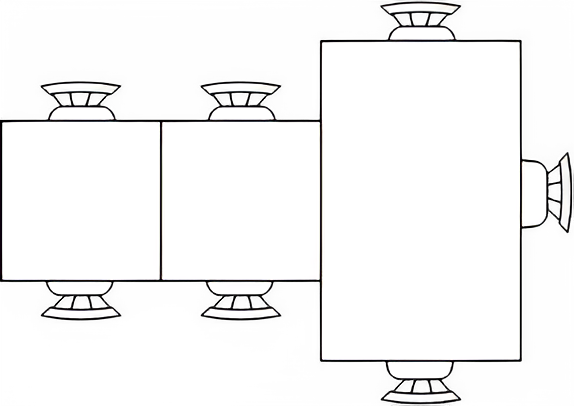
\includegraphics[width=10 cm]{images/tables.png}
	\label{fig:tables}
    \caption[Ground Truth Table Example]{The given ground truth considers these tables to be three distinct objects. Within the context of 
    plane detection, the three table tops would form exactly one plane.}
\end{figure}


\end{document}
